\documentclass[a4paper,11pt]{article}
\usepackage[margin=25mm]{geometry}
\usepackage[T1]{fontenc}
\usepackage{lmodern}
\usepackage{amsmath,amssymb,amsthm,graphicx,booktabs,float}
\usepackage[hidelinks]{hyperref}
\setlength{\emergencystretch}{3em}
\newtheorem{theorem}{Theorem}[section]
\newtheorem{lemma}[theorem]{Lemma}
\newtheorem{proposition}[theorem]{Proposition}
\newtheorem{corollary}[theorem]{Corollary}
\hypersetup{pdftitle={Frank-Wolfe under gap-dependent smoothness},pdfauthor={Yaroslav P. Lyakhov and Stepan A. Suvorov}}
\title{Frank-Wolfe under gap-dependent smoothness}
\author{Yaroslav P. Lyakhov \and Stepan A. Suvorov}
\date{14 November 2026 (revision v20)}
\begin{document}
\maketitle
\begin{abstract}
We study Frank-Wolfe under the constrained curvature condition
$\|\nabla^2f(x)\|\le L_0+L_1G(x)$, where $G$ is the full
Frank-Wolfe gap. We prove a transport bound along the selected direction,
an exponential upper model, and a logarithmic step with guaranteed descent.
The step uses neither the minimum value nor the quasar-convexity parameter.
For quasar-convex objectives, an accumulated computable lower bound gives
finite stopping and separates the $L_0/\varepsilon$ and
$L_1\log(1/\varepsilon)$ contributions.
We obtain linear convergence when $L_0=0$, and on strongly convex
domains with a nonzero gradient at the minimizer.
We establish the same order of update complexity for ordinary Armijo FW,
with additional function trials, and give data-derived constants for
multidimensional Poisson regression. We relate the model to known
gradient-norm smoothness and growth conditions. An exponential example
separates the explicit step from a fixed global-$L$ short step, although
ordinary endpoint steps solve that example immediately.
Comparisons on synthetic regression problems report separate oracle costs,
including cases where adaptive competitors are faster.
\end{abstract}
\section{Problem and available information}
The norm of the gradient need not vanish at a constrained minimum.
The full Frank-Wolfe gap accounts for the feasible directions and
does vanish there. We therefore use the gap in the curvature model,
derive a feasible descent step, and then use quasar-convexity to
convert descent into an objective-accuracy guarantee.

Let $Q\subset\mathbb R^n$ be nonempty, compact, and convex, with
$\operatorname{diam}Q\le D$, where $D>0$. Let $f$ be $C^2$ on a
neighborhood of $Q$, and fix a minimizer $x^*\in Q$.
All vector norms are Euclidean and matrix norms are spectral.
The available operations are evaluation of $f$, evaluation of its
gradient, and exact minimization of a linear function over $Q$.
At a current point $x$, compute
\begin{equation}\label{eq:gap}
 s\in\arg\min_{v\in Q}\langle\nabla f(x),v\rangle,\qquad
 d=s-x,\qquad
 G(x)=\langle\nabla f(x),x-s\rangle
     =\max_{v\in Q}\langle\nabla f(x),x-v\rangle.
\end{equation}
We assume
\begin{equation}\label{eq:gap_smoothness}
 \|\nabla^2f(x)\|\le L_0+L_1G(x)\quad(x\in Q),
 \qquad L_0,L_1\ge0.
\end{equation}
This condition depends on the feasible set. In particular,
$L_1D^2$ is dimensionless; the factor $D$ in the transport estimate
below cannot be dropped.

For convergence to the global minimum, we assume
$\gamma$-quasar-convexity about $x^*$:
\begin{equation}\label{eq:quasar}
 \gamma\bigl(f(x)-f(x^*)\bigr)
       \le\langle\nabla f(x),x-x^*\rangle\quad(x\in Q),
 \qquad 0<\gamma\le1.
\end{equation}
A convex objective satisfies this with $\gamma=1$. The condition
also admits nonconvex functions, as the example in Section~\ref{sec:examples}
shows. The step requires valid $L_0,L_1,D$; the objective-accuracy
test additionally uses $\gamma$. Neither $x^*$ nor $f(x^*)$ is an
input.

The constrained first-order condition gives $G(x^*)=0$, including
when $\nabla f(x^*)\ne0$. From \eqref{eq:gap} and \eqref{eq:quasar},
\begin{equation}\label{eq:certificate}
 0\le f(x)-f(x^*)\le \frac{G(x)}{\gamma}.
\end{equation}
Thus the gap bounds the objective error from above. Quasar-convexity
alone does not reverse this inequality.

\subsection{Relation to existing results and scope of the contribution}
The full gap and its use as an optimality certificate are standard~\cite{jaggi}.
The norm-dependent model and descent analysis of Vyguzov and
Stonyakin~\cite{vyguzov}, also published with Gasnikov~\cite{vyguzovjournal},
motivate our treatment of \eqref{eq:gap_smoothness}.
Mart\'{i}nez-Rubio~\cite{quasar} already studies constrained quasar-convex FW;
in particular, Theorem~9 gives $6LD^2/((k+1)\gamma^2)$ under ordinary
smoothness. Thus neither quasar-convex FW nor the factor $\gamma^{-2}$
is introduced here.

The accumulated certificate used below also has a known convex antecedent:
for $\gamma=1$ it is exactly the best primal-dual gap in
Wirth, Pe\~na, and Pokutta~\cite{wirth}, Section~2.2.
Their growth conditions relate the linear-model remainder to powers of $G$.
Section~\ref{sec:structure} gives an explicit connection to our assumption.
We use the certificate to analyze the proposed step for $0<\gamma\le1$;
we do not claim a new convex certificate.

Adaptive alternatives matter when comparing steps. Backtracking FW uses
objective tests to estimate curvature~\cite{pedregosa}; auto-conditioned FW
uses trial-point curvature without an inner search~\cite{acfw}.
Line-search-free conditional-gradient extensions also appear in
\cite{yagishita}. Adaptive Bregman steps handle a different, relative-smoothness
model~\cite{bregman}. These assumptions and guarantees are not identified
with \eqref{eq:gap_smoothness}.

\begin{table}[ht]
\centering\small
\caption{Position of the present analysis. Constants in different models
have different meanings; this is not a ranking of methods.}
\begin{tabular}{p{.23\linewidth}p{.34\linewidth}p{.34\linewidth}}
\toprule
Analysis & Curvature or growth information & Relevant distinction\\
\midrule
Norm-based FW~\cite{vyguzov} & $K_0+K_1\|\nabla f\|$ & Norm-dependent explicit short step\\
Quasar-convex FW~\cite{quasar} & Uniform $L$ & Known constrained quasar-convex rate\\
Open-loop FW~\cite{wirth} & Remainder controlled by $G^r$ & Known accumulated convex certificate\\
Adaptive FW~\cite{pedregosa,acfw} & Trial-point information & Does not require the supplied $L_0,L_1$\\
This analysis & $L_0+L_1G$ & Directional transport, explicit model minimizer, and certified stopping\\
\bottomrule
\end{tabular}
\end{table}

The contribution is the derivation and analysis of this particular curvature
model: a directional transport lemma, its logarithmic model minimizer,
separate $L_0/\varepsilon$ and $L_1\log(1/\varepsilon)$ contributions,
and verifiable examples. We also show that a conventional Armijo rule inherits
the same order of update complexity. The explicit rule saves trial function
evaluations when valid parameters are available; no universal numerical
advantage over adaptive FW is asserted.

\section{Two lemmas and a computable step}
The two lemmas in this section use \eqref{eq:gap_smoothness}
but do not require convexity or quasar-convexity of $f$.

\begin{lemma}[Transport and an upper model]\label{lem:transport}
Let $s,d$ be given by \eqref{eq:gap}. For $0\le t\le1$,
\begin{align}
 G(x+td)&\le(1-t)G(x)
    +D\|d\|\int_0^t\bigl(L_0+L_1G(x+ud)\bigr)\,du,
       \label{eq:transport}\\
 L_0+L_1G(x+td)&\le
      \bigl(L_0+L_1G(x)\bigr)e^{L_1D\|d\|t}.
       \label{eq:transport_exp}
\end{align}
Consequently, for $0\le\alpha\le1$,
\begin{equation}\label{eq:upper_model}
 f(x+\alpha d)\le f(x)-\alpha G(x)
 +(L_0+L_1G(x))\|d\|^2
       \int_0^\alpha(\alpha-t)e^{L_1D\|d\|t}\,dt.
\end{equation}
\end{lemma}
\begin{proof}
For every $v\in Q$, expand the inner product at $x$:
\[
 \langle\nabla f(x+td),x+td-v\rangle
 \le G(x)-tG(x)
       +D\|\nabla f(x+td)-\nabla f(x)\|.
\]
Maximizing over $v$ and integrating the Hessian along the segment
gives \eqref{eq:transport}. Drop the nonpositive term $-tG(x)$
and apply Gronwall's inequality to $L_0+L_1G(x+td)$ to obtain
\eqref{eq:transport_exp}; the case $L_1=0$ is immediate.
Taylor's formula with integral remainder gives \eqref{eq:upper_model},
since
$|d^\top\nabla^2f(x+td)d|\le\|\nabla^2f(x+td)\|\|d\|^2$.
\end{proof}

The exponential in \eqref{eq:upper_model} bounds the growth of
curvature while moving. The square $\|d\|^2$ comes from the second
directional derivative. Both arise in the proof; neither can be
removed by substituting the gap for a gradient norm in another model.
The selected segment is essential. For example,
$f(t)=t+t^3/6$ on $[0,1]$ has $|f''(t)|\le G(t)$, yet $G(0)=0$
and $f(1)>f(0)+f'(0)$. Thus an upper model with initial coefficient
$L_0+L_1G(x)$ cannot hold for \emph{every} pair $x,y$.

\paragraph{Step rule.}
If $G(x)>0$ and $L_1>0$, minimize the right-hand side of
\eqref{eq:upper_model} over $[0,1]$:
\begin{equation}\label{eq:log_step}
 \boxed{\displaystyle
 \alpha=\min\left\{1,\,
 \frac{1}{L_1D\|d\|}
 \log\left(1+
 \frac{L_1D\,G(x)}
 {(L_0+L_1G(x))\|d\|}\right)\right\}.}
\end{equation}
Here and below $\log$ is the natural logarithm.
If $L_1=0<L_0$, use the continuous limit
$\alpha=\min\{1,G(x)/(L_0\|d\|^2)\}$.
If $L_0=L_1=0$, use $\alpha=1$; $f$ is then affine on $Q$.
If $G(x)=0$, stop before evaluating any quotient.

\begin{lemma}[Descent]\label{lem:descent}
The step above satisfies
\begin{equation}\label{eq:descent}
 f(x+\alpha d)\le f(x)-\frac{\alpha G(x)}2.
\end{equation}
Outside the affine case,
\begin{equation}\label{eq:step_lower}
 \alpha\ge
 \min\left\{1,
   \frac{(\log2)G(x)}{(L_0+L_1G(x))D^2}\right\}.
\end{equation}
\end{lemma}
\begin{proof}
For this scalar calculation put $b=L_1D\|d\|>0$.
The integral in \eqref{eq:upper_model} equals
$(e^{b\alpha}-1-b\alpha)/b^2$.
Differentiating the model gives
\[
 -G(x)+(L_0+L_1G(x))\|d\|^2
             \frac{e^{b\alpha}-1}{b}.
\]
Its zero gives \eqref{eq:log_step}. At the capped minimizer
the derivative is nonpositive. Since $(e^{bt}-1)/b$ is convex
and vanishes at zero, its integral on $[0,\alpha]$ is at most
half of $\alpha$ times its endpoint value. Substitution in
\eqref{eq:upper_model} proves \eqref{eq:descent}.

For \eqref{eq:step_lower}, temporarily set
$r=\|d\|/D\le1$ and
$q=L_1G(x)/(L_0+L_1G(x))\le1$. The uncapped step is
$\log(1+q/r)/(L_1D^2r)$, and
\[
 \log(1+q/r)\ge\log(1+q)\ge q\log2\ge qr\log2.
\]
The middle inequality is concavity of the logarithm.
When $L_1=0$, both assertions follow from the quadratic model.
\end{proof}

In the norm-based step of~\cite{vyguzov}, a restriction on the
step length bounds an exponential by $e$.
Here \eqref{eq:log_step} solves the exponential model directly.
In particular, its logarithm makes
\[
 e^{L_1D\|d\|\alpha}-1
 \le\frac{L_1D\,G(x)}{(L_0+L_1G(x))\|d\|},
\]
which is precisely the inequality used in the descent proof.

\paragraph{Algorithm and stopping.}
Fix an accuracy $\varepsilon>0$.
At each visited point $x_k$, evaluate $f(x_k)$, its gradient,
and a full linear minimizer. Retain
\begin{equation}\label{eq:stop}
 \ell_k=\max_{0\le j\le k}
        \left\{f(x_j)-\frac{G(x_j)}{\gamma}\right\},
 \qquad \text{stop if } f(x_k)-\ell_k\le\varepsilon.
\end{equation}
Otherwise set $x_{k+1}=x_k+\alpha_kd_k$ using \eqref{eq:log_step}
or its stated limiting cases. Each new function value is evaluated
once. There is no line search.

\section{Stopping and convergence}
\label{sec:rates}
The step uses the observed gap and does not require $\gamma$.
The known value of $\gamma$ is needed for the lower bound in
\eqref{eq:stop}. Quasar-convexity gives
\begin{equation}\label{eq:retained_bound}
 0\le f(x_k)-f(x^*)\le f(x_k)-\ell_k\le G(x_k)/\gamma.
\end{equation}

\begin{theorem}[Finite certified stopping]\label{thm:gap_stopping}
Under \eqref{eq:gap_smoothness} and \eqref{eq:quasar}, the algorithm
stops with $f(x_N)-f(x^*)\le\varepsilon$.
If $G(x_0)>\gamma\varepsilon$, put
$J=\lceil\log_2(G(x_0)/(\gamma\varepsilon))\rceil$.
The number of updates satisfies
\begin{equation}\label{eq:gap_iteration_bound}
 N\le\left\lceil
 \frac{\max\{4,4L_1D^2/\log 2\}}{\gamma}\,J
 +\frac{16L_0D^2}{(\log 2)\gamma^2\varepsilon}
 \right\rceil.
\end{equation}
There are exactly $N+1$ objective evaluations, $N+1$ gradient
evaluations, and $N+1$ full linear minimizations, including the terminal
query. If $G(x_0)\le\gamma\varepsilon$, the algorithm stops immediately.
\end{theorem}
\begin{proof}
The affine case $L_0=L_1=0$ takes at most one full step.
Otherwise \eqref{eq:step_lower} and \eqref{eq:descent} imply
\begin{equation}\label{eq:gap_progress}
 f(x_k)-f(x_{k+1})\ge
 \min\left\{\frac{G(x_k)}2,
 \frac{(\log 2)G(x_k)^2}{2D^2(L_0+L_1G(x_k))}\right\}.
\end{equation}
The objective decreases and $\ell_k$ increases, so $f(x_k)-\ell_k$
decreases. Set $b_j=G(x_0)/(\gamma2^j)$ for $0\le j<J$ and assign
each nonterminal update to $b_j/2<f(x_k)-\ell_k\le b_j$.
In this phase, \eqref{eq:retained_bound} gives $G(x_k)>\gamma b_j/2$.
Since $t^2/(L_0+L_1t)$ increases for $t>0$, each such update decreases
the objective by at least
\[
 \min\left\{\frac{\gamma b_j}{4},
 \frac{(\log 2)\gamma^2b_j^2}{8D^2(L_0+L_1\gamma b_j/2)}\right\}.
\]
The total decrease from updates starting in the phase is at most the
true error at its entry, hence at most $b_j$. This includes the last
update leaving the phase, whose endpoint is still feasible.
The number of updates in the phase is therefore at most
\[
 \max\left\{\frac4\gamma,
 \frac{8L_0D^2}{(\log 2)\gamma^2b_j}
 +\frac{4L_1D^2}{(\log 2)\gamma}\right\}.
\]
Summation and $\sum_{j<J}b_j^{-1}<2/\varepsilon$ prove
\eqref{eq:gap_iteration_bound}. The same finite bound holds for every
unfinished prefix, excluding an infinite nonterminal run.
At each visited point the three oracles are called once; the explicit
step \eqref{eq:log_step} makes no trial objective calls.
\end{proof}

\subsection{The regime \texorpdfstring{$L_0=0$}{L0=0}}
\begin{corollary}[Geometric convergence]\label{cor:pure_gap_linear}
If $L_0=0<L_1$, set
\[
 \underline\alpha_0=\min\{1,(\log 2)/(L_1D^2)\}.
\]
For every computed iterate,
\begin{align*}
 f(x_k)-f(x^*)&\le
 (1-\gamma\underline\alpha_0/2)^k\bigl(f(x_0)-f(x^*)\bigr),\\
 f(x_k)-\ell_k&\le
 (1-\gamma\underline\alpha_0/2)^k G(x_0)/\gamma.
\end{align*}
If the initial test fails, stopping takes at most
\[
 \left\lceil\frac{\log(G(x_0)/(\gamma\varepsilon))}
 {-\log(1-\gamma\underline\alpha_0/2)}\right\rceil
\]
updates.
\end{corollary}
\begin{proof}
The step bound gives $\alpha_k\ge\underline\alpha_0$, so decrease
is at least $\underline\alpha_0G(x_k)/2$.
Use \eqref{eq:quasar} for the first recurrence and
\eqref{eq:retained_bound}, together with $\ell_{k+1}\ge\ell_k$,
for the second.
\end{proof}
Here $\nabla^2f(x^*)=0$ follows from $G(x^*)=0$.
The nonconvex example in Section~\ref{sec:examples} has this property
and a nonzero gradient at the minimum.

\subsection{Strongly convex feasible sets}
Use the convention of \cite{vyguzov}: $Q$ is strongly convex with
constant $\lambda>0$ if the closed ball of radius
$\lambda\|u-v\|^2$ about $(u+v)/2$ lies in $Q$ for all $u,v\in Q$.
This is a condition on the set, not strong convexity of the objective.

\begin{theorem}[A nonzero optimal gradient gives a linear rate]
\label{thm:strong_set_linear}
Suppose additionally that $Q$ is strongly convex and
$\nabla f(x^*)\ne0$. Then $x^*$ is unique and
\[
 c:=\min_{x\in Q}\|\nabla f(x)\|>0.
\]
Define
\[
 \underline\alpha_{\rm sc}=
 \min\left\{1,\left(\frac{L_0}{2\lambda c}+2L_1D^2\right)^{-1}\right\},
\]
with value $1$ when the denominator is zero. Then
\begin{align*}
 f(x_k)-f(x^*)&\le
 (1-\gamma\underline\alpha_{\rm sc}/2)^k
       \bigl(f(x_0)-f(x^*)\bigr),\\
 f(x_k)-\ell_k&\le
 (1-\gamma\underline\alpha_{\rm sc}/2)^k G(x_0)/\gamma.
\end{align*}
The algorithm uses neither $c$ nor $\lambda$; they enter only this rate.
\end{theorem}
\begin{proof}
If $y$ were another minimizer, \eqref{eq:quasar} would make
\[
 \frac{f(x^*+t(y-x^*))-f(x^*)}{t^\gamma}
\]
nondecreasing for $0<t\le1$. It is nonnegative and vanishes at $1$,
so the function is constant on the segment and
$\langle\nabla f(x^*),y-x^*\rangle=0$.
The midpoint ball and constrained first-order optimality instead give
\[
 \langle\nabla f(x^*),y-x^*\rangle
 \ge2\lambda\|\nabla f(x^*)\|\|y-x^*\|^2>0
\]
when $y\ne x^*$. Thus the minimizer is unique. A zero gradient anywhere
in $Q$ would give another minimizer by \eqref{eq:quasar}; continuity
and compactness now give $c>0$.

The same midpoint construction at a full linear minimizer yields
\[
 G(x_k)\ge2\lambda\|\nabla f(x_k)\|\|d_k\|^2
           \ge2\lambda c\|d_k\|^2.
\]
When $L_0=L_1=0$, $\alpha_k=1$. Otherwise,
$\log(1+t)\ge t/(1+t)$ in \eqref{eq:log_step}, or the stated limit
when $L_1=0$, gives
\[
 \alpha_k\ge\min\left\{1,
 \frac{G(x_k)}{(L_0+L_1G(x_k))\|d_k\|^2
                      +L_1D\|d_k\|G(x_k)}\right\}
 \ge\underline\alpha_{\rm sc}.
\]
Here $\|d_k\|\le D$ and the preceding scaling inequality bound the
denominator divided by $G(x_k)$ by $L_0/(2\lambda c)+2L_1D^2$.
The two recurrences follow as in Corollary~\ref{cor:pure_gap_linear}.
\end{proof}

\subsection{What an ordinary Armijo rule guarantees}\label{sec:armijo}
Consider the existing sufficient-decrease strategy: at each iterate start
with $\alpha=1$ and multiply it by a fixed $\beta\in(0,1)$ until
\begin{equation}\label{eq:armijo}
 f(x+\alpha d)\le f(x)-\alpha G(x)/2.
\end{equation}
Use the same accumulated certificate \eqref{eq:stop} and retain the
accepted function value. This rule requires neither $L_0,L_1$ nor $D$.
It is an ordinary Armijo search, not a new FW algorithm.

\begin{proposition}[Certified complexity of the Armijo comparator]
\label{prop:armijo}
Under the assumptions of Theorem~\ref{thm:gap_stopping}, let
$\alpha_{\log}(x)$ denote \eqref{eq:log_step}, including its limiting
cases. The search terminates and its accepted step satisfies
$\alpha\ge\beta\alpha_{\log}(x)$.
If $G(x_0)>\gamma\varepsilon$, its number of updates satisfies
\[
 N\le\left\lceil\frac1\beta\left[
 \frac{\max\{4,4L_1D^2/\log2\}}\gamma J
 +\frac{16L_0D^2}{(\log2)\gamma^2\varepsilon}
 \right]\right\rceil,
 \qquad J=\left\lceil\log_2\frac{G(x_0)}{\gamma\varepsilon}\right\rceil.
\]
Outside the affine case define
\[
 a_\varepsilon=\min\left\{1,
 \frac{(\log2)\gamma\varepsilon}
 {D^2(L_0+L_1\gamma\varepsilon)}\right\},\qquad
 T_\varepsilon=1+\left\lceil\frac{\log(1/a_\varepsilon)}{\log(1/\beta)}\right\rceil.
\]
There are $N+1$ gradient and LMO calls and at most $1+NT_\varepsilon$
function calls. In the affine case one trial suffices for the single
possible update.
\end{proposition}
\begin{proof}
The proof of Lemma~\ref{lem:descent} applies to every
$0<\alpha\le\alpha_{\log}(x)$: the model derivative is still
nonpositive and the same convex-integral bound proves \eqref{eq:armijo}.
The first grid point no larger than $\alpha_{\log}(x)$ is therefore
accepted unless a larger one has already passed. This proves termination
and the lower bound on the accepted step. The phase proof of
Theorem~\ref{thm:gap_stopping} now applies with every guaranteed decrease
multiplied by $\beta$.
Before stopping, $G(x)>\gamma\varepsilon$. Monotonicity of
$G/(L_0+L_1G)$ and \eqref{eq:step_lower} give
$\alpha_{\log}(x)\ge a_\varepsilon$, so at most $T_\varepsilon$ trials
are necessary. Each accepted function value is reused at the next point.
\end{proof}
When $L_0=0$, the certificate contracts by at least the factor
$1-\beta\gamma\underline\alpha_0/2$ per update. An analogous factor
$1-\beta\gamma\underline\alpha_{\rm sc}/2$ holds under
Theorem~\ref{thm:strong_set_linear}. Consequently, the favorable update
complexity is a consequence of the curvature assumption, not an
exclusive property of the logarithmic formula. Its specific benefit
is the guaranteed step without rejected function trials.

\section{Scope of the curvature condition}\label{sec:structure}
\subsection{Uniform smoothness and the gradient-norm model}
Since $f$ is $C^2$ near a compact $Q$, the uniform bound
$L=\max_{x\in Q}\|\nabla^2f(x)\|$ is finite. Our assumption is useful
through its parameters and the resulting local model, not because it admits
functions without a finite smoothness constant on this fixed $Q$.
Moreover,
\[
 G(x)\le D\|\nabla f(x)\|,
 \qquad \|\nabla^2f(x)\|\le L_0+(L_1D)\|\nabla f(x)\|.
\]
Thus gap-dependent smoothness implies a norm-dependent bound on $Q$.
The converse with the same zero constant term fails: $f(t)=e^t$ on
$[0,R]$ satisfies $|f''|=|f'|$, whereas $G(0)=0$ and $f''(0)=1$.
Every admissible gap-dependent pair therefore has $L_0\ge1$ in that example.
In general $L_0\ge\|\nabla^2f(x^*)\|$.

\begin{proposition}[A restriction of the pure-gap regime]\label{prop:rigidity}
Suppose \eqref{eq:gap_smoothness} holds with $L_0=0$.
If $\nabla f(z)=0$ at any $z\in Q$, then $\nabla f=0$ on $Q$ and
$f$ is constant on $Q$. Convexity or quasar-convexity of $f$ is not needed.
\end{proposition}
\begin{proof}
Fix $y\in Q$ and set $u(t)=\|\nabla f(z+t(y-z))\|$.
The fundamental theorem of calculus and $G\le D\|\nabla f\|$ give
\[
 u(t)\le L_1D\|y-z\|\int_0^t u(s)\,ds.
\]
Gronwall's inequality yields $u=0$. Varying $y$ proves the assertion.
\end{proof}
Consequently, a nonconstant problem in the pure-gap regime cannot have
a minimizer with zero gradient. In particular, an interior minimizer of a
full-dimensional feasible set is excluded. This restriction should be kept
in mind when interpreting Corollary~\ref{cor:pure_gap_linear}.

\subsection{Connection to existing growth conditions}
For convex $f$, write
$D_f(y,x)=f(y)-f(x)-\langle\nabla f(x),y-x\rangle$.
If $L_0=0<L_1$, Lemma~\ref{lem:transport} implies, for $0\le\alpha\le1$,
\[
 D_f(x+\alpha d,x)
 \le \frac{M\alpha^2}{2}G(x),
 \qquad M=L_1D^2e^{L_1D^2}.
\]
Indeed, bound the exponential in \eqref{eq:upper_model} by
$e^{L_1D^2}$ and integrate $\alpha-t$.
This is the strong $(M,1)$-growth condition used in~\cite{wirth}.
The reduction is conservative: it introduces an exponential dependence on
$L_1D^2$, whereas Corollary~\ref{cor:pure_gap_linear} uses an explicit
step lower bound of order $\min\{1,(L_1D^2)^{-1}\}$.
This comparison concerns the displayed conversion of constants, not a
lower bound on what all other analyses or algorithms can achieve.

\subsection{A multidimensional class with explicit parameters}
Let $a_i\in\mathbb R^n$, $y_i\ge0$, and $B=\max_i\|a_i\|>0$.
Consider the Poisson negative log-likelihood, up to data-only constants,
\begin{equation}\label{eq:poisson}
 f(x)=\frac1m\sum_{i=1}^m\bigl(e^{a_i^Tx}-y_i a_i^Tx\bigr),
 \qquad 0\in Q.
\end{equation}
For integer $y_i$ this is a count-regression objective; the following
bound also holds for nonnegative real responses.

\begin{proposition}[Parameters from the observed data]\label{prop:poisson}
On any compact convex $Q$ containing zero, \eqref{eq:poisson} satisfies
\eqref{eq:gap_smoothness} with
\begin{equation}\label{eq:poisson_constants}
 L_0=B^2\left(1+\frac{1}{2m}\sum_i y_i^2\right),
 \qquad L_1=B^2,\qquad \gamma=1.
\end{equation}
These constants do not require a minimizer or a minimum value.
If $Q=\{x:\|x\|\le R\}$, valid norm-dependent constants are
$K_0=L_0$, $K_1=RL_1$, and a uniform Hessian bound is
\begin{equation}\label{eq:poisson_uniform}
 L=e^{BR}\|A\|_2^2/m,
\end{equation}
where the rows of $A$ are $a_i^T$. These are valid bounds, not claims
of smallest possible constants.
\end{proposition}
\begin{proof}
For $y\ge0$ and $t\in\mathbb R$,
\begin{equation}\label{eq:poisson_scalar}
 e^t\le 1+y^2/2+t(e^t-y).
\end{equation}
For $t\le0$, $(1-t)e^t+yt\le1$.
For $t\ge0$, the derivative of $(1-t)e^t$ is $-te^t\le-t$, so
$(1-t)e^t+yt\le1-t^2/2+yt\le1+y^2/2$.
Also $\|\nabla^2f(x)\|\le B^2m^{-1}\sum_i e^{a_i^Tx}$.
Summing \eqref{eq:poisson_scalar} therefore gives
\[
 \|\nabla^2f(x)\|\le L_0+L_1\langle\nabla f(x),x\rangle
 \le L_0+L_1G(x),
\]
where the last step uses $0\in Q$.
On a ball, $\langle\nabla f(x),x\rangle\le R\|\nabla f(x)\|$.
Finally $a_i^Tx\le BR$ implies
$\nabla^2f(x)\preceq e^{BR}A^TA/m$.
\end{proof}
The ball's linear oracle is $s=-R\nabla f(x)/\|\nabla f(x)\|$
when the gradient is nonzero. It generally differs from the minimizer
of \eqref{eq:poisson}. Thus these problems avoid the endpoint degeneracy
of the scalar examples below. The model and parameter bounds are global
on $Q$; the numerical experiments only sample their consequences.

\section{Examples and a quantitative comparison}\label{sec:examples}
\subsection{Gap-dependent constants and a large uniform constant}
Let
\begin{equation}\label{eq:exp_family}
 f_A(x,y)=e^x+Ay,\qquad
 Q=[0,R]\times[0,1],\qquad R,A>0,\qquad D=\sqrt{R^2+1}.
\end{equation}
This function is convex, its minimum is at $(0,0)$, and
$\nabla f_A(0,0)=(1,A)$.
The full linear minimizer is $(0,0)$, so
\[
 G(x,y)=xe^x+Ay,\qquad
 \|\nabla^2 f_A(x,y)\|=e^x\le1+xe^x\le1+G(x,y).
\]
Indeed, $(1-x)e^x$ is nonincreasing for $x\ge0$ and equals one
at zero. Thus $L_0=L_1=1$ work for every $R,A$, whereas the
smallest uniform Hessian bound on $Q$ is $L=e^R$.

\begin{theorem}[Two step rules on the same family]\label{thm:separation}
Start both methods at $(R,0)$ in \eqref{eq:exp_family}.
If continued without an earlier positive-tolerance stop, the
logarithmic rule \eqref{eq:log_step} reaches the exact minimum
in at most
\begin{equation}\label{eq:exp_upper}
 N_{\log}\le\left\lceil\frac{R\sqrt{R^2+1}}{\log2}\right\rceil
\end{equation}
updates. For the ordinary short step
$\alpha=\min\{1,G/(L\|d\|^2)\}$ with $L=e^R$,
attaining objective error at most $\varepsilon>0$ requires
\begin{equation}\label{eq:exp_lower}
 N_L\ge\frac{e^R/(1+\varepsilon)-1}{e-1}.
\end{equation}
The iterates, steps, objective values, gaps, certificates, and
operation counts are independent of $A$.
\end{theorem}
\begin{proof}
Every iterate has $y=0$. For the logarithmic rule its first coordinate
satisfies
\[
 x_{\mathrm{next}}=\max\{0,x-h(x)\},\qquad
 h(x)=\frac1D\log\left(1+\frac{D}{x+e^{-x}}\right).
\]
On $[0,R]$, $x+e^{-x}\le R+e^{-R}\le D$. The last inequality
follows from $e^R-e^{-R}\ge2R$, whose left-hand side has derivative
at least two.
Thus $h(x)\ge(\log2)/D$, which proves \eqref{eq:exp_upper}.

For the ordinary short step, write
$x_{\mathrm{next}}=x-h$, where $h=\min\{x,e^{x-R}\}\le1$.
Convexity of the exponential on $[0,1]$ gives
\[
 e^{-(x-h)}-e^{-x}
 =e^{-x}(e^h-1)
 \le(e-1)e^{-x}h\le(e-1)e^{-R}.
\]
Initially $e^{-x}=e^{-R}$. Error at most $\varepsilon$ requires
$e^{-x}\ge1/(1+\varepsilon)$, which proves \eqref{eq:exp_lower}.
On $y=0$, all function values, gaps, directions, and step formulas
are independent of $A$; hence so is \eqref{eq:stop}.
\end{proof}

At fixed accuracy, these bounds compare a quadratic upper bound
in $R$ with an exponential lower bound for the specified uniform-$L$
step. The small numbers $L_0,L_1$ matter through the proved step
and work estimates, not through a numerical comparison of constants
with different units.

\paragraph{What this comparison does not establish.}
The linear oracle returns the global minimizer for every point in
\eqref{eq:exp_family}. Thus the ordinary schedule $\alpha_k=2/(k+2)$,
indexed from $k=0$, reaches the minimizer in one update; so does exact
line search. Theorem~\ref{thm:separation} is a separation of two specified
step rules, not a complexity lower bound for FW in general or evidence
of superiority over adaptive competitors. Varying $A$ from the start
$(R,0)$ adds no trajectory diversity: this is a one-dimensional control
of sensitivity to a normal gradient component.

\subsection{A nonconvex objective with a nonzero optimal gradient}
On $Q=[0,1]$, consider
\begin{equation}\label{eq:nonconvex}
 f(x)=\int_0^x e^{-2t^2}\,dt.
\end{equation}
The minimizer is $x^*=0$, $f'(0)=1$, and $f''(x)<0$ for $x>0$.
Moreover,
\[
 G(x)=xe^{-2x^2},\qquad
 |f''(x)|=4G(x),\qquad
 xf'(x)\ge e^{-2}x\ge e^{-2}f(x).
\]
Thus \eqref{eq:gap_smoothness} holds with $L_0=0,L_1=4$,
and \eqref{eq:quasar} holds with $\gamma=e^{-2}$.
This is a nonconvex member of the stated class.

From $x_0=1$, the first logarithmic step gives
$x_1=1-(\log2)/4\in(1/2,1)$.
Since $xe^{-2x^2}$ decreases with $x$ on $(1/2,1]$,
$G(x_1)>G(x_0)$ even though $f(x_1)<f(x_0)$.
This explains why the stopping proof uses the monotone quantity
$f(x_k)-\ell_k$ rather than assuming monotonicity of $G(x_k)$.
The gradient norm increases toward one as the iterates approach
the constrained minimum.

Here too the linear oracle returns the minimizer $0$ and exact line search
selects the full step. The purpose of this example is to verify membership
in a nonconvex pure-gap class and the nonmonotonicity of $G$, not to
demonstrate a difficult numerical problem.

\section{Reproducible numerical comparisons}\label{sec:experiments}
\subsection{Analytical controls retained from the initial study}
The fixed controls use \eqref{eq:exp_family} with
$R\in\{1,2,4,6,8\}$, $A\in\{1,1000\}$, start $(R,0)$, and
$\varepsilon=10^{-6}$. Both short-step methods use \eqref{eq:stop}
with $\gamma=1$. Gap-log uses $L_0=L_1=1$ and Global-$L$ uses the
smallest uniform bound $L=e^R$. The choices of $A$ give identical
trajectories, not independent instances. Table~\ref{tab:endpoint}
includes the endpoint comparators needed to interpret this control.
\begin{table}[ht]
\centering
\caption{Updates on the exponential control. The last column follows
from the oracle returning the minimizer. A terminal point query
certifies termination.}\label{tab:endpoint}
\begin{tabular}{rrrr}
\toprule
$R$ & Gap-log & Global-$L$ & Open-loop / exact line search\\
\midrule
1 & 2 & 1 & 1\\
2 & 5 & 6 & 1\\
4 & 17 & 52 & 1\\
6 & 35 & 400 & 1\\
8 & 60 & 2976 & 1\\
\bottomrule
\end{tabular}
\end{table}
Four further controls use \eqref{eq:nonconvex}, $f(x)=x+x^2/2$
on $[0,1]$ from $1$, $f(x)=x$ on the same interval from $1$, and
\eqref{eq:exp_family} with $R=4,A=1000$ starting at $(0,0)$.
They take $5,1,1,0$ updates. All 24 historical runs pass the original
checks. Their summary values reproduce; some trajectory entries differ
in the last floating-point digits across environments. No cross-platform
byte identity of numerical traces is claimed.

\subsection{Protocol for multidimensional regression}
We use \eqref{eq:poisson} over Euclidean balls. For
$n\in\{4,12\}$ and seeds $11,29,47$, draw $m=12n$ independent
standard Gaussian rows and normalize each to unit Euclidean norm.
Draw a further Gaussian vector and scale its norm to $1.2$; call it
$b$. Generate integer counts $y_i\sim\operatorname{Poisson}(e^{a_i^Tb})$.
Use radii $R\in\{0.5,2,4\}$ and starts $0,Re_1,-Re_1$.
The six datasets, three radii and three starts give 18 constrained
problems and 54 starting configurations. Radii and starts sharing data
are dependent conditions, not independent statistical samples.

All methods use \eqref{eq:stop}, $\gamma=1$, $\varepsilon=10^{-4}$,
and a cap of 20,000 outer attempts. Parameters are fixed in
\texttt{Code/benchmark\_multidim.py} and written to the protocol file
before execution. The matrices and counts are saved.
Proposition~\ref{prop:poisson} supplies gap and norm parameters;
\eqref{eq:poisson_uniform} supplies the uniform bound.
These bounds are not tuned after observing performance.

Eight rules are compared. Gap-log uses \eqref{eq:log_step};
Global-$L$ uses $\min\{1,G/(L\|d\|^2)\}$; Open-loop uses $2/(k+2)$.
Armijo starts at $1$ and halves until \eqref{eq:armijo} holds.
Backtracking uses the quadratic-model test of~\cite{pedregosa},
with initial estimate $M=1$, per-iteration initial trial $M/2$,
and doubling on failure. Norm-based uses
$\min\{1,G/[e(K_0+K_1\|\nabla f\|)\|d\|^2]\}$ from~\cite{vyguzov}.
Line bisection checks the endpoint derivative, then bisects a
sign-changing bracket to width $10^{-12}$; it approximates exact
line search. AC-FW implements Algorithms~1--2 and damping (6),
with $\delta=1$, of~\cite{acfw}; its compulsory initial LMO move is
charged and may increase the objective. The implementations are
independent of the cited authors' software.

Function, full-gradient and LMO counters increment on every actual call.
Rejected function trials and gradients used in bisection are counted.
Accepted function values are reused; after an AC rejection the unchanged
gradient and atom are reused. No solver receives an optimum.
Separately, SLSQP gives a diagnostic interval $[f(z)-G(z),f(z)]$;
its largest computed width is $2.75\cdot10^{-7}$.
Seven of the 18 reference solutions are on the boundary and eleven
are interior according to the recorded tolerance. These are
floating-point diagnostics, not exact optimality proofs.

\subsection{Results and computational costs}
There are 432 recorded solver runs. Gap-log and six other methods
converge in all 54 configurations; Open-loop reaches the cap in nine,
all with $n=4,R=4$. The unfinished final certificates range from
$1.07\cdot10^{-4}$ to $1.80\cdot10^{-4}$ and remain in all summaries.
Table~\ref{tab:costs} reports medians over all 54 configurations,
including capped endpoints. The costs of a capped method must not
be interpreted as guaranteed costs to convergence.

\begin{table}[ht]
\centering\small
\caption{Recorded costs: successes, updates $N$, function calls $F$,
gradient calls $H$, LMO calls $V$, and milliseconds.
Time is first the median of three sequential untraced repetitions
per configuration, then the median across configurations;
validation and file output are excluded.}\label{tab:costs}
\begin{tabular}{lrrrrrr}
\toprule
Rule & Success & $N$ & $F$ & $H$ & $V$ & ms\\
\midrule
\csname @@input\endcsname multidim_table.tex
\bottomrule
\end{tabular}
\end{table}

\begin{table}[ht]
\centering\small
\caption{Median recorded updates at each radius, across 18 starting
configurations. All capped Open-loop runs belong to $R=4$.}
\label{tab:radius}
\begin{tabular}{lrrr}
\toprule
Rule & $R=0.5$ & $R=2$ & $R=4$\\
\midrule
\csname @@input\endcsname radius_table.tex
\bottomrule
\end{tabular}
\end{table}

At $R=4$, Gap-log improves on the supplied uniform bound in median
updates (216.5 versus 819), whereas the uniform rule is cheaper at
the two smaller radii. Backtracking and AC-FW are substantially cheaper
than Gap-log on this collection. Armijo uses fewer gradients and LMOs
but pays for repeated function trials; line bisection uses many gradients.
Separating oracle types changes the interpretation of update counts.
The experiment supports limitations of a fixed global bound in some
regimes, but not superiority over adaptive alternatives.

\begin{figure}[ht]
\centering
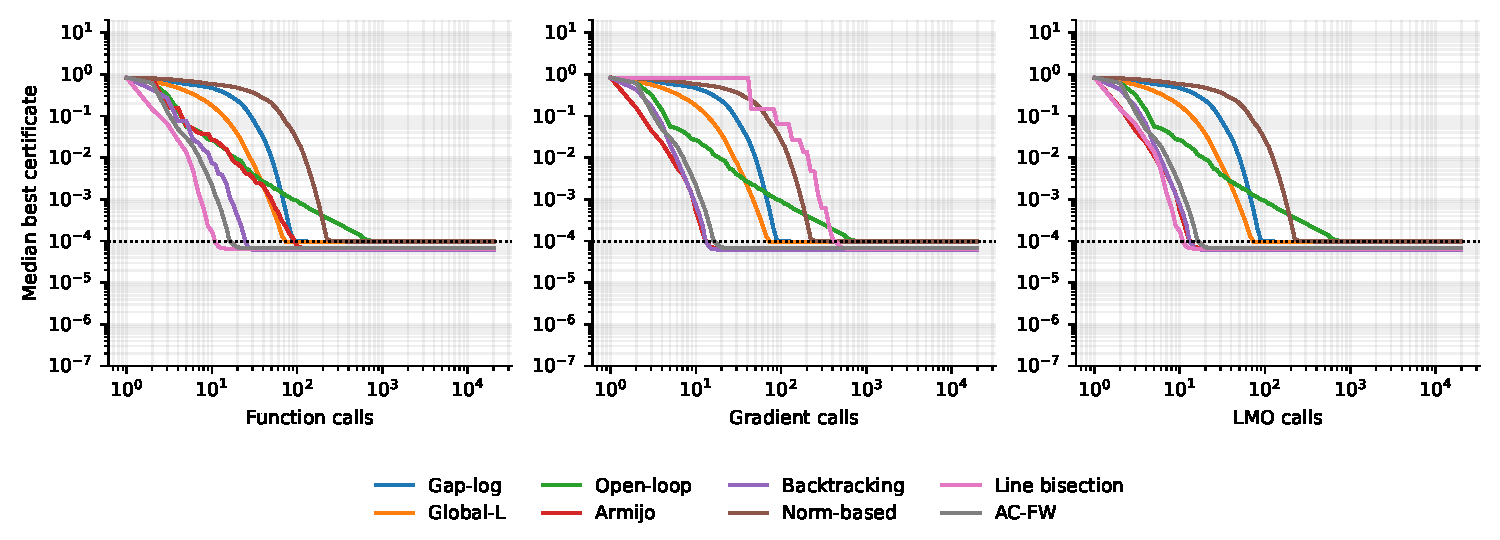
\includegraphics[width=\linewidth]{figures/multidim_en.pdf}
\caption{Median best recorded certificate versus separate oracle budgets
over the same 54 configurations. Values after termination or the run cap
are held at the last best recorded value. The dotted line is $10^{-4}$.
The panels use different cost units, which are not added together.}
\label{fig:cost_curves}
\end{figure}

\paragraph{Reproduction and validation.}
\texttt{Code/benchmark\_gap.py} reproduces the historical controls;
\texttt{Code/benchmark\_multidim.py} records multidimensional iterates,
parameters, statuses and counters.
\texttt{Code/report\_results.py} generates tables and figures from saved
data without solving new problems.
The trace audit checks feasibility, lower-bound consistency with the
diagnostic intervals, applicable descent and step bounds, and oracle
accounting on 340,433 recorded points. Hessian bounds are sampled at
up to 25 points per run; their global justification is
Proposition~\ref{prop:poisson}, not this sampling.
Eight separate tests check derivatives by finite differences, the scalar
inequality, scaling, actual interface calls, initial stopping, Armijo
trials, bisection and a nonoptimal oracle endpoint.
The 13 historical symbolic identities also pass.
Dependencies and commands are included in the accompanying archive.

\section{Limitations and interpretation}
The guarantees assume exact gradients and full linear minimization.
Approximate or stochastic oracles require additional error terms and are
not covered here. The logarithmic step needs valid $L_0,L_1,D$; a certified
objective-accuracy test additionally needs a valid $\gamma$.
Proposition~\ref{prop:poisson} supplies these quantities for a concrete
class, but does not make their verification automatic for arbitrary models.

The compact-domain assumptions already imply ordinary smoothness.
The relevant question is whether exploiting the gap-dependent parameters
is useful, not whether a global $L$ exists. Proposition~\ref{prop:rigidity}
also limits the pure-gap regime: it cannot describe a nonconstant problem
with a zero-gradient minimizer. The nonzero-gradient assumption in
Theorem~\ref{thm:strong_set_linear} is substantive.

The experiments concern small synthetic regression instances, and the
global and norm-dependent constants are valid analytical bounds rather
than optimized constants. Timing depends on hardware and implementation.
The results do not establish broad superiority, optimal dependence on
$\gamma$, or matching lower bounds for the proposed complexity estimate.
Proposition~\ref{prop:armijo} shows explicitly that a familiar adaptive
rule shares its order in accepted updates. The contribution is a
parameter-explicit analysis of gap-dependent curvature and a model-minimizing
step with no rejected function evaluations.

\paragraph{Use of computational tools.}
AI tools assisted with derivations, checks, implementation, and writing.
The authors are responsible for the mathematical claims and reported results.
Symbolic identities, floating-point controls, and mathematical proofs are
reported separately; no formal proof-assistant certification is claimed.

\begin{thebibliography}{99}
\bibitem{jaggi}M.~Jaggi.
Revisiting Frank-Wolfe: Projection-Free Sparse Convex Optimization.
\emph{Proceedings of the 30th International Conference on Machine Learning},
PMLR 28(1):427-435, 2013.
\url{https://proceedings.mlr.press/v28/jaggi13.html}.

\bibitem{vyguzov}A.~A.~Vyguzov and F.~S.~Stonyakin.
Frank-Wolfe Algorithms for $(L_0,L_1)$-smooth functions.
\href{https://arxiv.org/abs/2510.16468v5}{arXiv:2510.16468v5}, 2026.

\bibitem{vyguzovjournal}A.~A.~Vyguzov, F.~S.~Stonyakin, and A.~V.~Gasnikov.
Frank-Wolfe algorithms for $(L_0,L_1)$-smooth functions.
\emph{Journal of Nonlinear and Variational Analysis} 10(3):597--616, 2026.
\href{https://doi.org/10.23952/jnva.10.2026.3.05}{doi:10.23952/jnva.10.2026.3.05}.

\bibitem{quasar}D.~Mart\'{i}nez-Rubio.
Fast Quasar-Convex Optimization with Constraints.
\emph{Proceedings of the 29th International Conference on
Artificial Intelligence and Statistics}, PMLR 300:3340-3348, 2026.
\url{https://proceedings.mlr.press/v300/martinez-rubio26a.html}.

\bibitem{wirth}E.~Wirth, J.~Pe\~na, and S.~Pokutta.
Adaptive open-loop step-sizes for accelerated convergence rates of the
Frank--Wolfe algorithm.
\emph{Computational Optimization and Applications} 95:679--698, 2026.
\href{https://doi.org/10.1007/s10589-026-00817-w}{doi:10.1007/s10589-026-00817-w}.

\bibitem{pedregosa}F.~Pedregosa, G.~N\'{e}giar, A.~Askari, and M.~Jaggi.
Linearly Convergent Frank-Wolfe with Backtracking Line-Search.
\emph{AISTATS}, PMLR 108:1--10, 2020.
\url{https://proceedings.mlr.press/v108/pedregosa20a.html}.

\bibitem{acfw}K.-H.~Giang-Tran, S.~Shafiee, and N.~Ho-Nguyen.
Auto-Conditioned Frank-Wolfe Algorithms.
\href{https://arxiv.org/abs/2605.15512v2}{arXiv:2605.15512v2}, 2026.

\bibitem{bregman}S.~Takahashi, S.~Pokutta, and A.~Takeda.
Fast Frank--Wolfe Algorithms with Adaptive Bregman Step-Size for Weakly
Convex Functions. \emph{ICLR}, 2026.
\url{https://arxiv.org/abs/2504.04330}.

\bibitem{yagishita}S.~Yagishita and M.~Ito.
Simple linesearch-free first-order methods for nonconvex optimization.
\href{https://arxiv.org/abs/2509.14670}{arXiv:2509.14670}, 2025.
\end{thebibliography}

\end{document}
